\documentclass[12pt]{report}
\usepackage{amsthm, amssymb}
\usepackage{geometry}
\geometry{legalpaper,  margin=1in}
\usepackage{amsmath}
\usepackage{enumitem}

\newtheorem*{remark}{Remark}
\newtheorem{theorem}{Theorem}
\newtheorem{corollary}{Corollary}[theorem]
\newtheorem{lemma}[theorem]{Lemma}
\newtheorem*{defi}{Definition}
\newtheorem{ex}{Example}
\usepackage{xcolor}
\usepackage{graphicx}

\newcommand{\R}{\mathbb{R}^2}
\newcommand{\x}{\mathbf{x}}
\newcommand{\y}{\mathbf{y}}
\newcommand{\m}{\text{max}}
\title{Topology HW 7}
\author{Ben Kallus}
\date{Due Friday. April 2, 2021}

\begin{document}

\maketitle

\noindent Draw a unit ball using the square metric, $B_\rho(x,\varepsilon)$. Next draw a unit ball using the Euclidean metric,  $B_d(x, \varepsilon)$. Explain how you got these two sets. 

\begin{center} 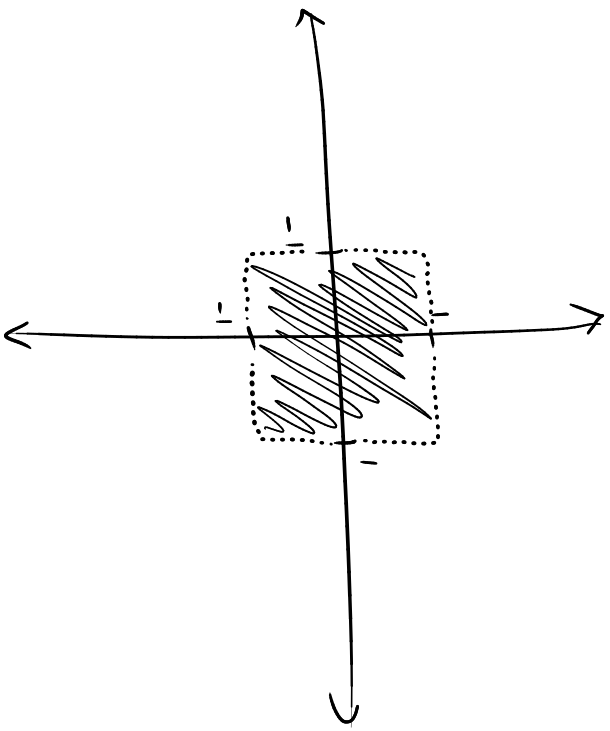
\includegraphics[angle=90,scale=.4]{square.png} \end{center}
	The plot above shows the unit ball using the square metric because every point within the square with side length 2 centered at the origin has at least one dimension with absolute value less than 1.

\begin{center} 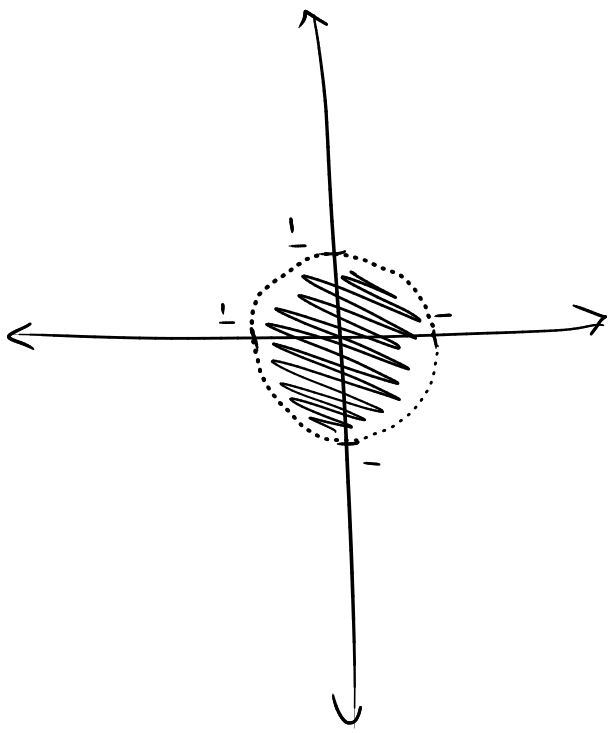
\includegraphics[angle=90,scale=.4]{circle.png} \end{center}
	The plot above shows the unit ball using the Euclidean metric because every point within the unit circle satisfies $x^2 + y^2 < 1$, and thus has Euclidean distance less than 1 from the origin.

\newpage 

\begin{theorem}[Theorem 20.3 for $\R$ ]
The topologies on $\R$ induced by the Euclidean metric $d$ and the square metric $\rho$ are the same as the product topology on $\R$
\end{theorem}
\begin{proof}
Let $\x = (x_1,x_2)$ and $\y= (y_1,y_2)$ be points in $\R$. Then
\begin{eqnarray*}
\rho(\x, \y) &=&  \m \{ \vert x_1- y_1 \vert , \vert x_2- y_2 \vert \} \\
&\leq& \left(  \vert x_1 -y_1 \vert^2 +\vert x_2 -y_2 \vert^2 \right)^{1/2}\\ &=& d(\x,\y)\\
&\leq& \left(  (\m \{ \vert x_1- y_1 \vert , \vert x_2- y_2 \vert \} )^2 +(\m \{ \vert x_1- y_1 \vert , \vert x_2- y_2 \vert \} )^2 \right)^{1/2}\\
&=& (\rho(\x,\y)^2+ \rho(\x,\y)^2)^{1/2}\\ 
&=& \sqrt{2} \rho(\x,\y).
\end{eqnarray*}
Therefore, we have 
\begin{equation}
\rho(\x,\y) \leq d(\x,\y) \leq \sqrt{2}\rho(\x,\y).
\end{equation}
\emph{We will first show that the topology induced by $d$ and $\rho$ are the same.}\\\\
Let $\y \in B_d(\x, \varepsilon)$ we have $d(\x,\y) < \varepsilon$ and so $\rho(\x,\y) \leq d(\x,\y) < \varepsilon$ and so $\y \in B_\rho (\x, \varepsilon)$. Therefore, $B_d(\x, \varepsilon) \subset B_\rho(\x, \varepsilon)$. 


\begin{center}
	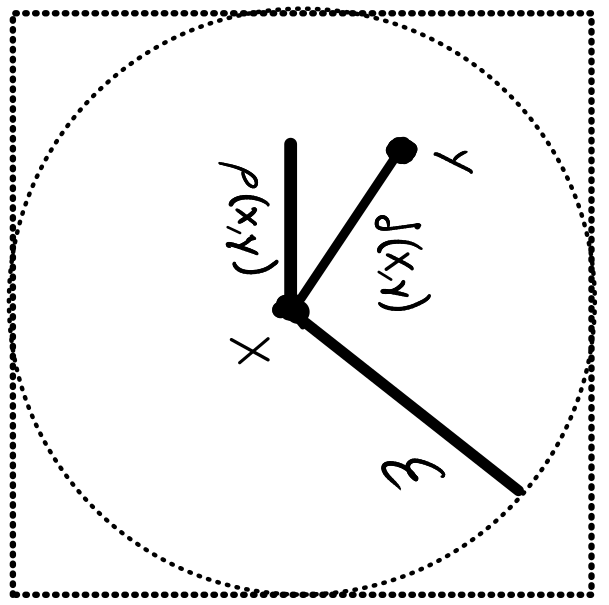
\includegraphics[scale=.5,angle=90]{pic1.png}
\end{center}
By Lemma 20.2, the metric topology induced by $d$ is finer than the metric topology induced by $\rho$.

Let $\y \in B_\rho(\x, \varepsilon/\sqrt{2})$ we have $\rho(\x,\y) < \varepsilon/\sqrt{2}$ and by (\ref{ine}) we know $d(\x,\y) \leq \sqrt{2}\rho(\x, \y) = \sqrt{2} (\varepsilon/\sqrt{2}) = \varepsilon$. This means that $\y \in B_d(\x, \varepsilon)$. Therefore, $B_\rho(\x, \varepsilon/\sqrt{2}) \subset B_d(\x, \varepsilon)$. 
\begin{center}
{\color{red}Include a picture that illustrates what we just did.}
\end{center}
\vspace{2in}
By Lemma 20.2 we have that the metric topology induced by $\rho $ is finer than the metric topology induced by $d$. 

Hence, the metric topologies induced by $\rho$ and $d$ are the same on $\R$.
\\\\
\emph{We now show that the product topology and the metric topology induced by $\rho$ are the same.}\\\\

Let $B = (a_1,b_1) \times (a_2,b_2)$ be a basis element for the product topology on $\R$. Let $\x = (x_1, x_2) \in B$. Then  $x_i \in (a_i, b_i)$ for each $i =1,2$ and we have $\varepsilon_i = \text{min}\{ x_i - a_i, b_i - x_i\}$. Set $\varepsilon = \text{min} \{ \varepsilon_1 , \varepsilon_2 \}$. Then 
\[ B_\rho (\x, \varepsilon) \subset (x_1-\varepsilon_1 , x_1+ \varepsilon_1) \times (x_2-\varepsilon_2 , x_2+ \varepsilon_2) \subset B. \]

\begin{center}
{\color{red}Include a picture that illustrates what we just did.}
\end{center}
\vspace{2in}
By Lemma 13.3, the metric topology induced by $\rho$ is finer than the product topology.

Conversely, let $B_\rho (\x, \varepsilon)$. Let 

\[B= B_\rho(\x, \varepsilon) = (x_1 - \varepsilon , x_1 + \varepsilon) \times (x_2 - \varepsilon, x_2 + \varepsilon).\]
In this case $B$ is already a basis element for the product topology and so $B \subset B_\rho(\x, \varepsilon)$. By Lemma 13.3, the product topology is finer than the metric topology induced by $\rho$. 

Therefore, all three topologies are the same on $\R$.

\end{proof}

\newpage\noindent\textbf{2)} Proposition: The Euclidean metric on $\mathbb R^2$ is a metric.
\begin{proof}
	Let $\mathbf x, \mathbf y \in \mathbb \R^2$.
	Observe that
	\begin{align*}
		d(\mathbf x, \mathbf y) &= \sqrt{(x_1-y_1)^2 + (x_2-y_2)^2} \\
					&= \sqrt{(y_1-x_1)^2 + (y_2-x_2)^2} \\
					&= d(\mathbf y, \mathbf x).
	\end{align*}

	Suppose that $\mathbf x, \mathbf y \in \mathbb R^2$ such that $d(\mathbf x, \mathbf y) = 0$.
	Then,
	\begin{align*}
		\sqrt{(x_1-y_1)^2 + (x_2-y_2)^2} &= 0, \\
		\implies (x_1-y_1)^2 + (x_2-y_2)^2 &= 0, \\
		\implies (x_1-y_1)^2 &= -(x_2-y_2)^2.
	\end{align*}

	Since $(x_1-y_1)^2$ is positive and $-(x_2-y_2)^2$ is negative, it must be that both are 0.
	Thus, $x_1 = y_1$ and $x_2 = y_2$, so $\mathbf x = \mathbf y$.

	Let $\mathbf z \in \mathbb R^2$.
	Then,
	\begin{align*}

\end{proof}


\end{document}

